% !TeX spellcheck = en_GB

\section{Information Retrieval I}

\begin{breakbox}
\boxtitle{IR Definition:}
\begin{itemize}
	\item Finding unstructured and semi- structured data in large amount of documents based on a users information need.
	\item A modern computer science perspective, i.e. algorithms, techniques and tools.
\end{itemize}
\end{breakbox}

\begin{breakbox}
\boxtitle{Basic Text Matching:}
\lstinputlisting[language=SQL]{sql_code/regex_ts_vector.sql}
\end{breakbox}

\begin{breakbox}
\boxtitle{Wild card queries:}
\begin{itemize}
	\item mon*: find all docs containing any word beginning mon.
	\item Easy with binary tree (or B-tree) lexicon: retrieve all words in range: mon $\leq$ w $<$ moo
	\item *mon: find words ending in mon: harder (Maintain an B-tree for terms backwards).
	\item Bigram (k-gram, sequence of k chars) indexes (Maintain a second inverted index from bigrams to dictionary terms that match each bigram).
\end{itemize}
Code: See above.
\end{breakbox}

\begin{breakbox}
	\boxtitle{Overview of different text search methods}
	\begin{center}
		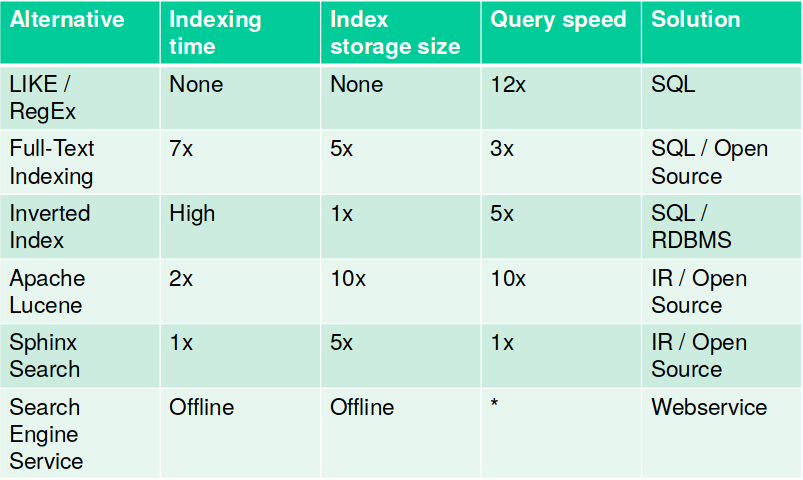
\includegraphics[width=0.16\textwidth]{slides_images/text_search_methods}
	\end{center}
\end{breakbox}

\begin{breakbox}
\boxtitle{Data vs. Information Retrieval:}
\begin{itemize}
	\item Data Retrieval:
		\begin{itemize}
			\item which docs contain a set of keywords?
			\item well defined semantics.
			\item not error tolerant: a single erroneous object implies failure!
		\end{itemize}
	\item Information Retrieval:
		\begin{itemize}
			\item information about a subject or topic.
			\item semantics is frequently loose.
			\item small errors are tolerated.
			\item IR differs conceptually from database queries!
		\end{itemize}
\end{itemize}
\end{breakbox}

\begin{breakbox}
\boxtitle{Inverted Index (Inverted List):}
\begin{itemize}
	\item For each term T, we must store a list of all documents that contain T.
	\item Linked lists generally preferred to arrays.
\end{itemize}
\begin{center}
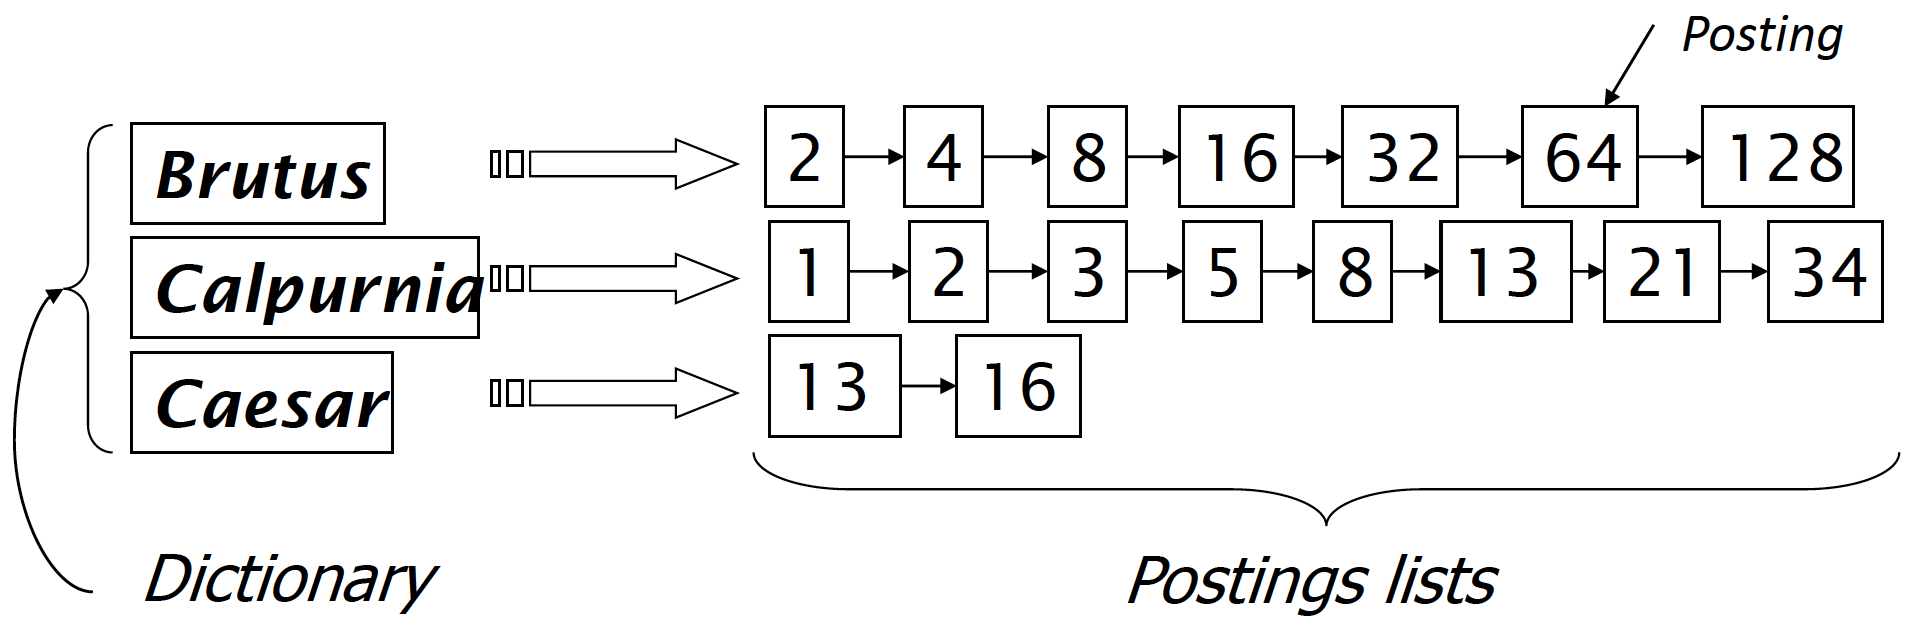
\includegraphics[width=.15\textwidth]{slides_images/inverted_index}
\end{center}
Term Frequency Matrix:
\begin{center}
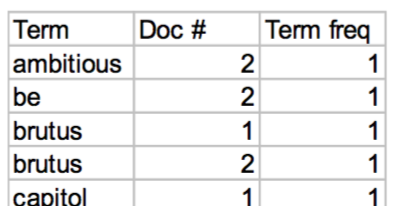
\includegraphics[width=.05\textwidth]{slides_images/term_frequency_matrix}
\end{center}
The following properties are often used when constructing an inverted index:
\begin{description}
	\item[Tokenization] Split the document into segments. Mostly words.
	\item[Normalization/Stemming] Cuts irrelevant parts from words. Seen $\implies$ See.
	\item[Lemmatization] Stemming with more context. Saw $\implies$ See.
	\item[Stopp words] Words which should not be added to the index.
	\item[Special compound words] A German language problem. E.g. ''Naturschutzobjekt''.
\end{description}
\end{breakbox}

\begin{breakbox}
\boxtitle{Full Text To Index Terms:}
\newline Logical view of the documents.
\begin{center}
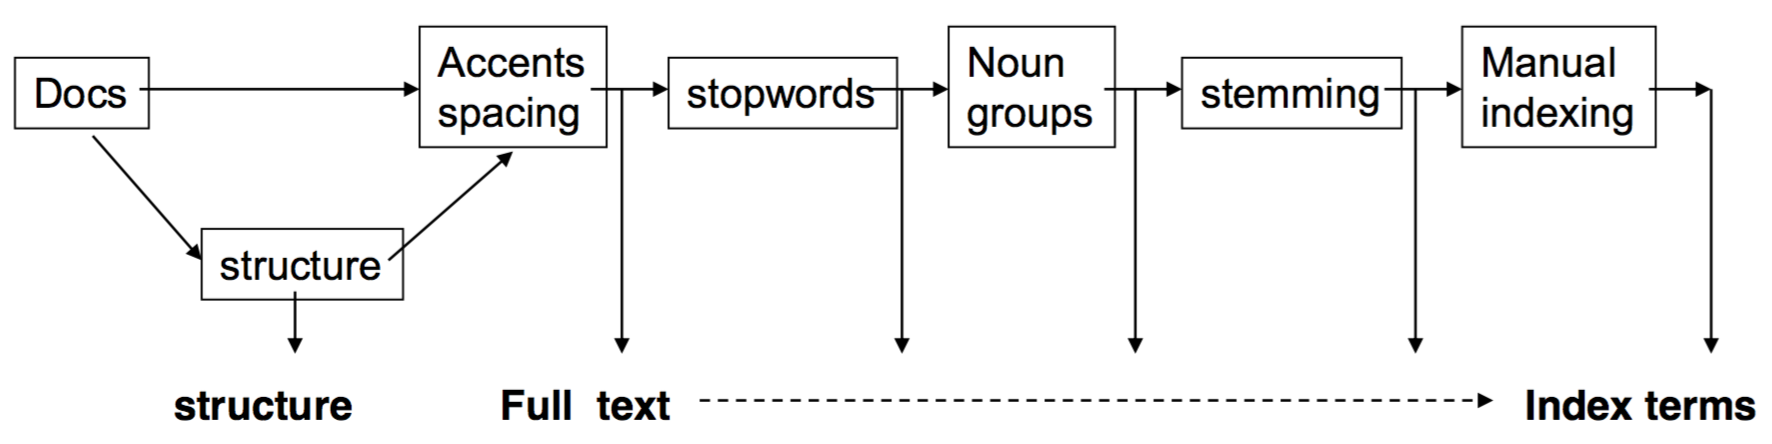
\includegraphics[width=.15\textwidth]{slides_images/full_to_index}
\end{center}
\end{breakbox}

\begin{breakbox}
\boxtitle{IR-Models:}
\begin{center}
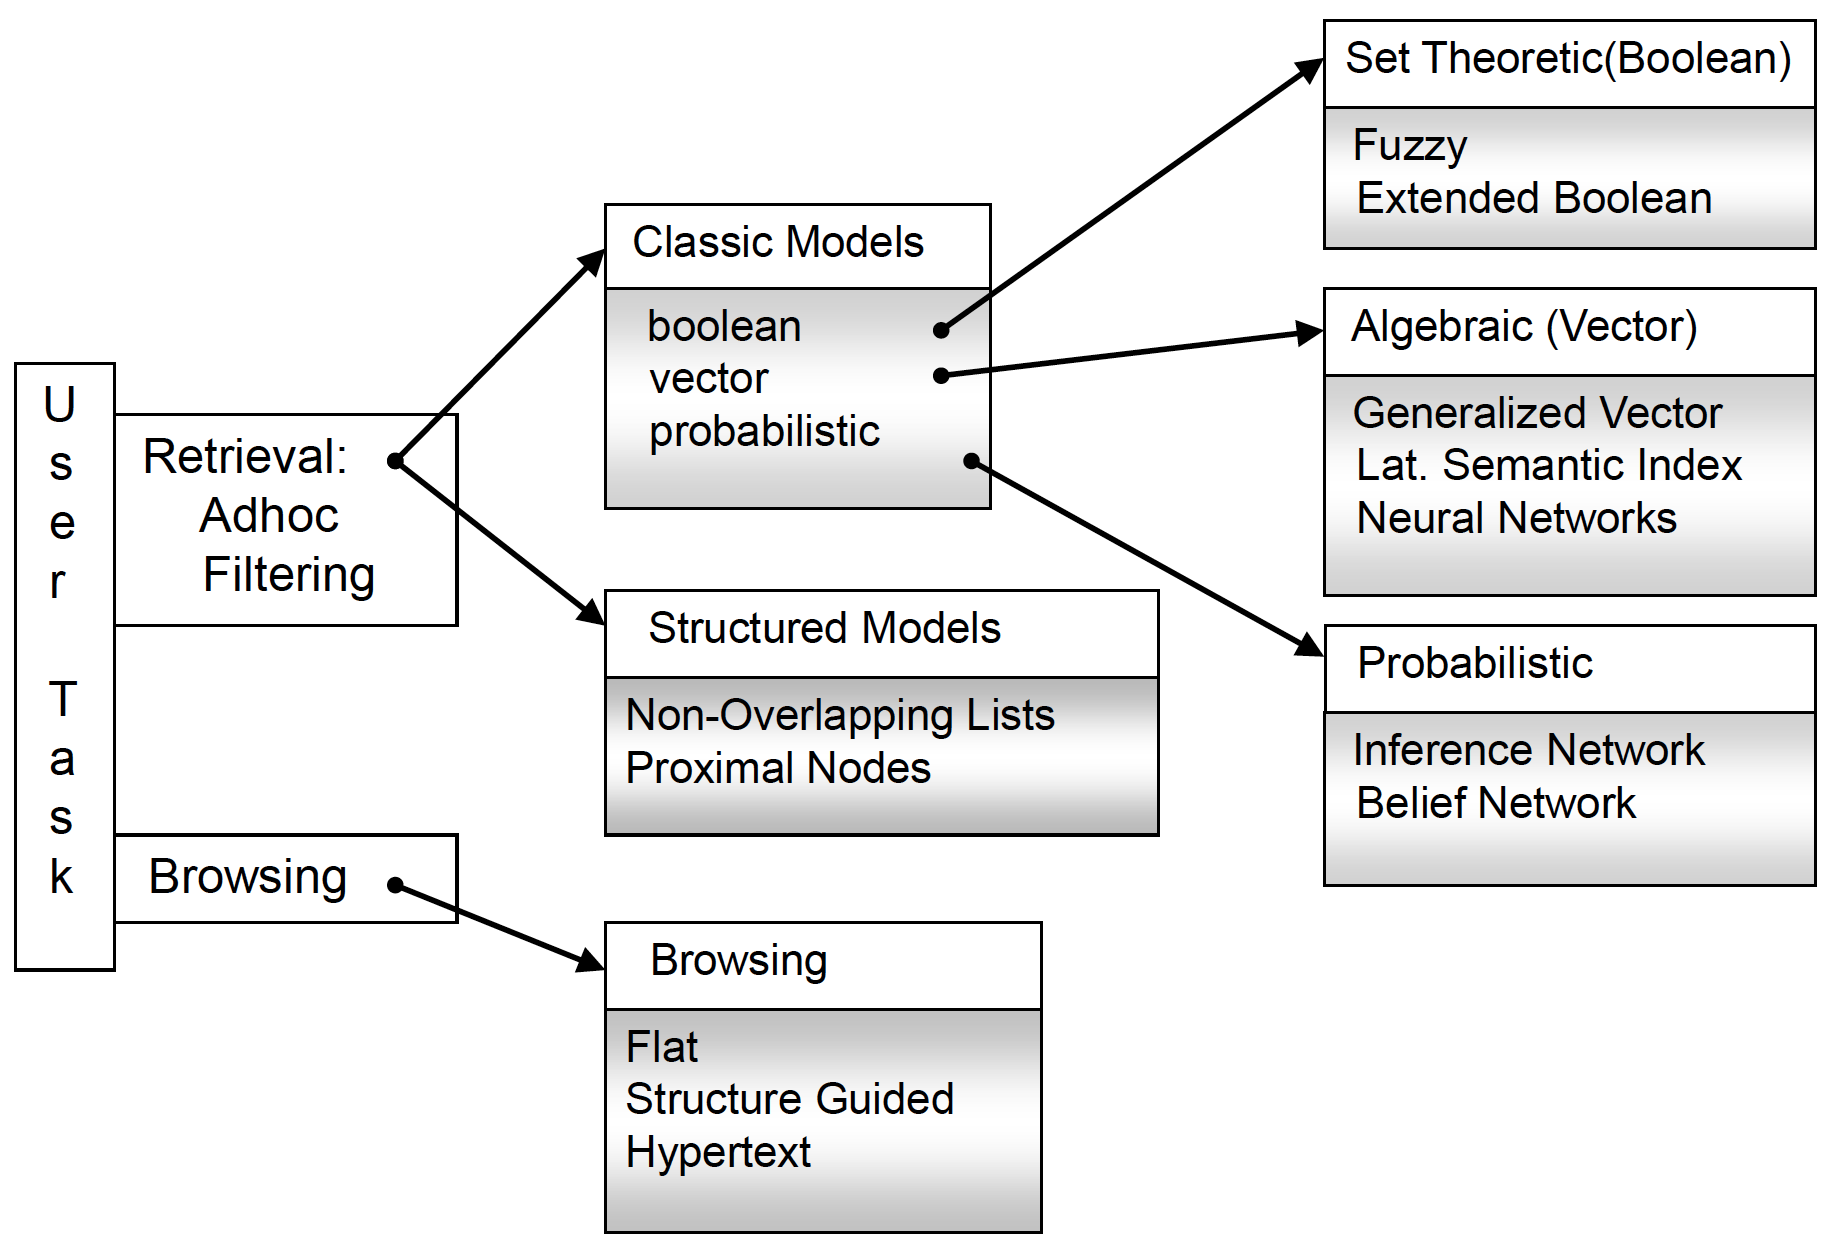
\includegraphics[width=.15\textwidth]{slides_images/ir_models}
\end{center}
\end{breakbox}
